
\documentclass[11pt,a4paper,oneside]{article}
\usepackage[T1]{fontenc} 
\usepackage[utf8]{inputenc}
\usepackage[main=english]{babel}
\usepackage{graphicx} % 1pt = 0.035146cm
\usepackage[justification=default]{subfig} %Manage sub-figures 
\usepackage[update]{epstopdf}
\usepackage[labelfont=bf]{caption}
\usepackage{titlesec} % Allows customization of titles
\usepackage{booktabs}
\usepackage{wrapfig}

\usepackage{color}
\usepackage[textwidth = 450pt,top = 80pt, bottom = 60pt]{geometry}
\usepackage{soul}
\newcommand{\hlc}[2][yellow]{{\sethlcolor{#1}\hl{#2}}}
\usepackage[inline]{enumitem}
\usepackage[symbol]{footmisc}

\renewcommand{\thefootnote}{\fnsymbol{footnote}}

%--------------------------------------------------------------------------------
%       MATH PACKAGES
%--------------------------------------------------------------------------------
\usepackage{amsmath}
%\usepackage{mathtools}
\usepackage[leqno,fleqn,intlimits]{empheq}
\usepackage{bm}
%\usepackage{amssymb}
\usepackage{empheq}

%--------------------------------------------------------------------------------
%       MATLAB CODE
%--------------------------------------------------------------------------------
\usepackage{mcode}
%--------------------------------------------------------------------------------
%       MY COMMANDS
%--------------------------------------------------------------------------------
\renewcommand{\vec}[1]{\mathbf{#1}}
\newcommand{\tr}{\textcolor{red}}
\newcommand{\mathbi}[1]{\bm{\textbf{\em #1}}}
%--------------------------------------------------------------------------------
%       BIBLIOGRAPHY PACKAGES
%--------------------------------------------------------------------------------
% \usepackage{csquotes}
% \usepackage[sorting=nyt,%
% sortcites=true,%
% bibencoding=ascii,%
% autopunct=true,%
% hyperref=true,%
% language=auto,%
% %backref=true,%
% url=false,%
% maxcitenames=10,%
% minbibnames = 3,%
% maxbibnames=3,%
% giveninits, 
% natbib = false,
% isbn=false,%
% backend=biber]{biblatex}
% \addbibresource{bibliograhy_assignment.tex}
%--------------------------------------------------------------------------------
%       MISCELLANEA
%--------------------------------------------------------------------------------
\usepackage[]{hyperref}
\usepackage{cleveref}
%%% CREF setup
\crefname{equation}{Eq.}{Eqs.}
\crefname{table}{Table}{Tables}
\crefname{figure}{Fig.}{Figs.}

%--------------------------------------------------------------------------------
%       TITLE SECTION
%--------------------------------------------------------------------------------
\newcommand\headlinecolor{\normalcolor}

\makeatletter
\renewcommand*\maketitle{%
    \begingroup
    \centering
    \fontsize{15}{15}% 72pt on 80pt leading
    \selectfont
    \headlinecolor
    \@title\\
    \vspace{5mm}
    \@author
    \par
    \vskip1in
    \endgroup
    \vspace{-22mm}
}
\makeatother


\title{MSAS -- Assignment \#1: Simulation} % Article title
\author{\large {Lorenzo Cucchi}, {123456}}
\date{}

%--------------------------------------------------------------------------------
% HEADING packages
\usepackage{fancyhdr} % Headers and footers control
\setlength{\headheight}{15.2pt}
\pagestyle{fancyplain} % Defines a new header for all pages (absolutely all pages, use fancy to exclude title-page and chapters, if book class is used) 
\fancyhf{} % clears the header and footer, otherwise the elements of the default "plain" page style will appear
%
\lhead{{Lorenzo Cucchi}, MSAS -- Assignment \#1}
\rhead{\vspace{-0.5cm}
\includegraphics[width=0.3\textwidth]{newlogo.eps}}
\lfoot{AY 2023-24 -- Prof.\ F.\ Topputo; TA: C.\ Balossi, S.\ Borgia}
\rfoot{\thepage}
%--------------------------------------------------------------------------------
%       BEGIN DOCUMENT
%--------------------------------------------------------------------------------
\begin{document}

\maketitle

\thispagestyle{fancy}

\section{Implicit equations}

\subsection*{Exercise 1}

Let $\vec{f}$ be a two-dimensional vector-valued function $\vec{f}(\vec{x}) = (x_2^2-x_1-2, \ -x_1^2+x_2+10)^\top$, where $\vec{x} = (x_1, x_2)^\top$. Find the zero(s) of $\vec{f}$ by using Newton's method with $\partial\vec f/\partial\vec x$ 
\begin{enumerate*}[label=\arabic*)]
    \item computed analytically, and
    \item estimated through finite differences.
\end{enumerate*}
Which version is more accurate?

\rightline{\small(3 points)}
\medskip  \hrule \medskip


\begin{figure}[h]
    \centering
    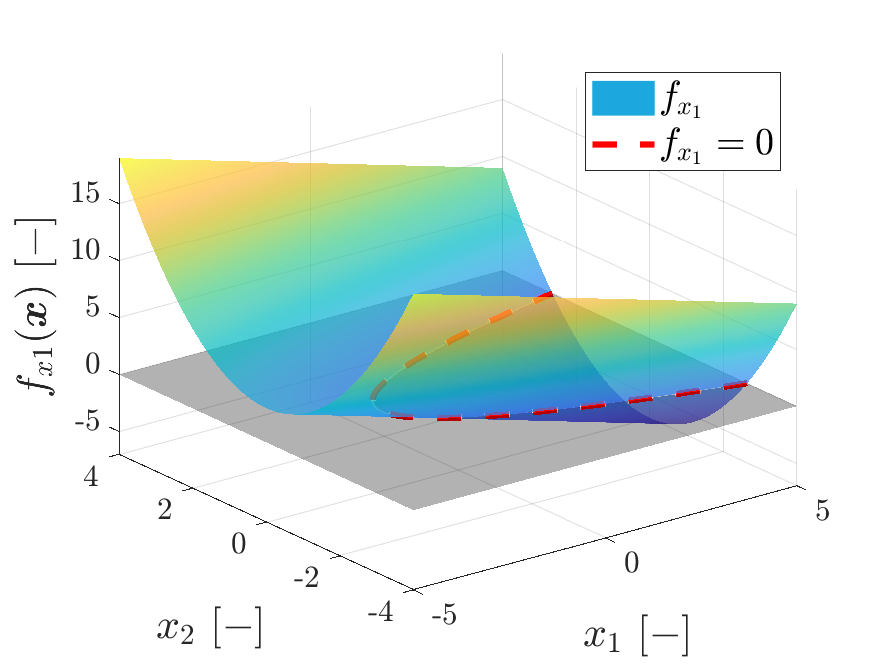
\includegraphics[width = 0.48\textwidth]{gfx/ex1_1.pdf}
    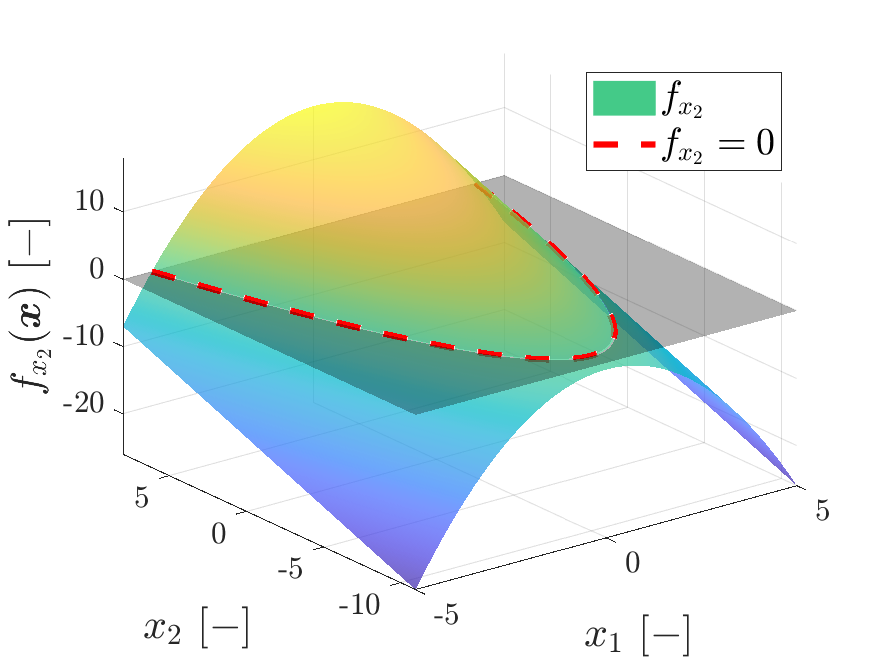
\includegraphics[width = 0.48\textwidth]{gfx/ex1_2.pdf}
    \caption{Surf plot of function $f_x(\vec{x})=x_1^2+x_2-5$ (left) and function $f_y(\vec{x})=x_2^2-x_1$ (right).}
    \label{fig:f1f2}
\end{figure}
The problem consists in finding the couple(s) $\{x_1, x_2\}$ which satisfy the relation $f(x_1,x_2)=[0, 0]^T$. In order to solve the problem using Newton's method, the analytical form or an approximation of the inverse Jacobian matrix $\vec{J^{-1}}$ is needed. In fact, according to Newton's method, the i-th iteration $\vec{x}_{i}$ is given by \autoref{eq:Jacobian}.
\begin{equation}
    \vec{x}_{i} = \vec{x}_{i-1} - \vec{J^{-1}}(\vec{x}_{i-1}) \vec{f}(\vec{x}_{i-1})
    \label{eq:Jacobian}
\end{equation}

\begin{wrapfigure}[17]{r}{0.5\textwidth}
\centering
\vspace{-0.3cm}
    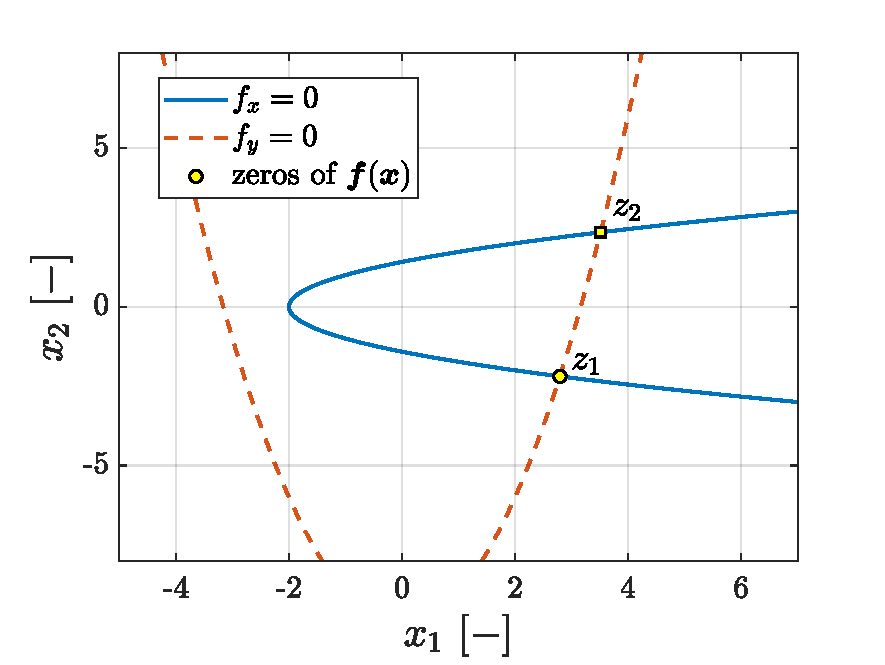
\includegraphics[width = 0.5\textwidth]{gfx/ex1_3.pdf}
    \caption{Zeros ($z_1$ and $z_2$) of the problem.}
    \label{fig:ex1_solution}
\end{wrapfigure}
The analytical form of the inverse Jacobian matrix is easily obtained through MATLAB symbolic toolbox after a few passages. On the other side, the approximated form of the Jacobian matrix is obtained through finite difference methods. In particular, first order \textit{forward} and \textit{centered} finite difference schemes are implemented. In this sense, the small increment $\delta$ which is applied in the finite difference methods follows the \textit{golden rule}: $\delta=\sqrt{eps}\cdot max(1, |\vec{x}|)$, where $eps$ is the machine epsilon. Furthermore, to improve code efficiency and accuracy, the Jacobian calculated with finite differences in never inverted; instead, the MATLAB command \texttt{backslash} "$\backslash$" is used.

As \autoref{fig:ex1_solution} shows, there are two zeros of the function $\vec{f}$($\vec{x}$). Indeed, two appropriate initial guesses $\vec{x}_0$ must be found to make the algorithms converge at the two zeros. The initial guesses are therefore $x_{0,1}=[0, 2]^T$ and $x_{0,2}=[6, -4]^T$. The stopping criteria chosen is the accuracy of the function evaluated in $\vec{x}_i$: when both the absolute values of $f_x(\vec{x}_i)$ and $f_y(\vec{x}_i)$ are lower than a tolerance set to $1e-8$ the algorithm stops.
Results reported in \autoref{tab:ex1_results} show that the three algorithms converge at very close values and take the same number of iterations: the error $||err||=||\vec{f}(\vec{x}_{end,analytical}) - \vec{f}(\vec{x}_{end,method})||$ is very low, suggesting the high accuracy of both the forward and centered differences approximations.
\begin{table}[ht]
    \centering
    \begin{tabular}{l|c c c}
        \textbf{Method} & \mbox{\boldmath $z_1$} & \textbf{Iterations} &  \mbox{\boldmath $||err||$} \\
        \midrule
        \midrule
        Analytical                  & [2.794695112889339, -2.189679226029504]$^T$  & 5 & -\\
        Forward differences         & [2.794695112889365, -2.189679226029504]$^T$  & 5 & 4.1405e-14\\
        Centered differences        & [2.794695112889314, -2.189679226029504]$^T$  & 5 & 2.6291e-14\\
        \toprule
    \end{tabular}
    \begin{tabular}{l|c c c}
        \textbf{Method} & \mbox{\boldmath $z_2$} & \textbf{Iterations} &  \mbox{\boldmath $||err||$} \\
        \midrule
        \midrule
        Analytical                  & [3.513999235947622, 2.348190630240421]$^T$  & 5 & -\\
        Forward differences         & [3.513999235947627, 2.348190630240434]$^T$  & 5 & 1.3773e-14\\
        Centered differences        & [3.513999235947620, 2.348190630240424]$^T$  & 5 & 3.1401e-15\\
    \end{tabular}
    \caption{Zeros found by the three proposed methods.}
    \label{tab:ex1_results}
\end{table}

%--------------------------------------------------------------------------------
%       IMPLICIT EQUATION
%--------------------------------------------------------------------------------




\clearpage

%--------------------------------------------------------------------------------
%       NUMERICAL SOLUTION OF NONLINEAR ODE
%--------------------------------------------------------------------------------

\section{Numerical solution of ODE}
\subsection*{Exercise 2}

The Initial Value Problem $\dot x = x- 2t^2+2$, $x(0) = 1$, has analytic solution $x(t) = 2t^2 + 4t - e^t + 2$. 
\begin{enumerate*}[label=\arabic*)]
    \item Implement a general-purpose, fixed-step Heun's method (RK2);
    \item Solve the IVP in $t\in[0,2]$ for $h_1 = 0.5$, $h_2 = 0.2$, $h_3 = 0.05$, $h_4 = 0.01$ and compare the numerical vs the analytical solution;
    \item Repeat points 1)--2) with RK4;
    \item Trade off between CPU time \& integration error.
\end{enumerate*}

\rightline{\small(4 points)}
\medskip \hrule \medskip

\begin{figure}[ht]
    \centering
    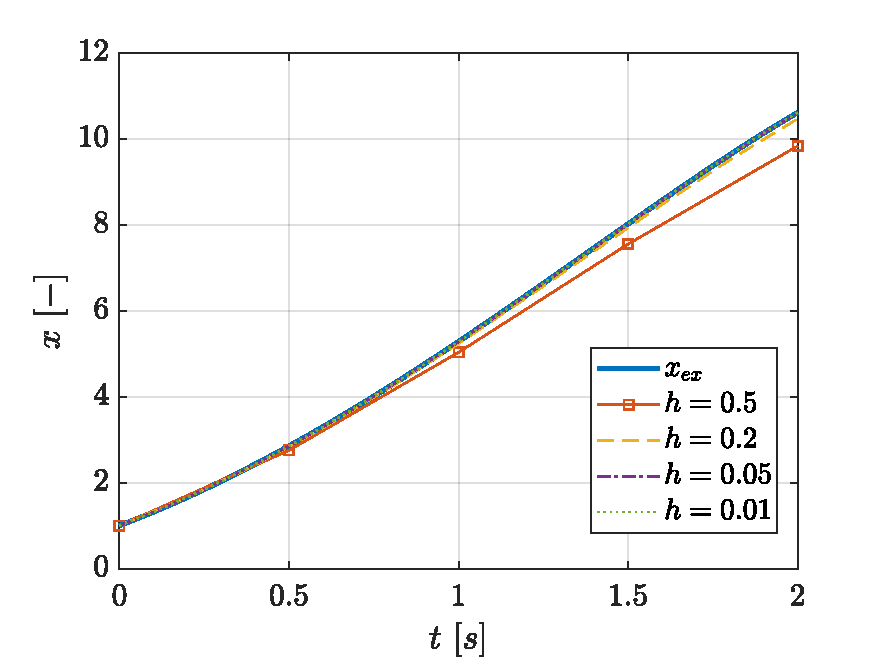
\includegraphics[width = 0.48\textwidth]{gfx/ex2_1.pdf}
    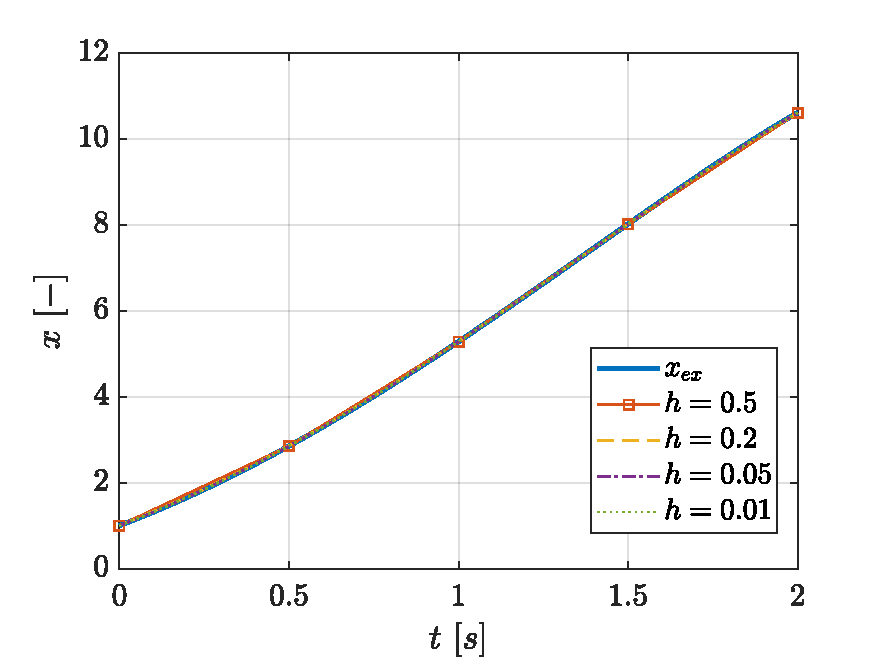
\includegraphics[width = 0.48\textwidth]{gfx/ex2_2.pdf}
    \caption{Solutions provided by with $RK2$ (left) and $RK4$ (right) methods by varying $h$ value.}
    \label{fig:ex2_sol}
\end{figure}

The IVP problem in $t\in[0,2]$ for $h_1 = 0.5$, $h_2 = 0.2$, $h_3 = 0.05$ and $h_4 = 0.01$ is 
first solved with RK2 and RK4 methods, as shown in (\autoref{fig:ex2_sol}), and then, the 
integration errors are compared in \autoref{fig:ex2_locErr}. As depicted in the two figures, 
the accuracy of the RK4 method is higher w.r.t. RK2 one, even with higher values of $h$. 
The higher order of the RK4 method grants also an higher decrease order for the global 
integration error, as shown in \autoref{fig:ex2_globErr} (left figure).

By taking into consideration the trade-off between computational time and integration error, 
the \autoref{fig:ex2_globErr} (right) shows that to accomplish the same accuracy on the final 
value the RK4 method needs less time w.r.t. RK2 method. Indeed, the user should use RK4 method 
regardless of the computational time since it is the most efficient on both the accuracy and 
CPU-time needed.

\begin{figure}[ht]
    \centering
    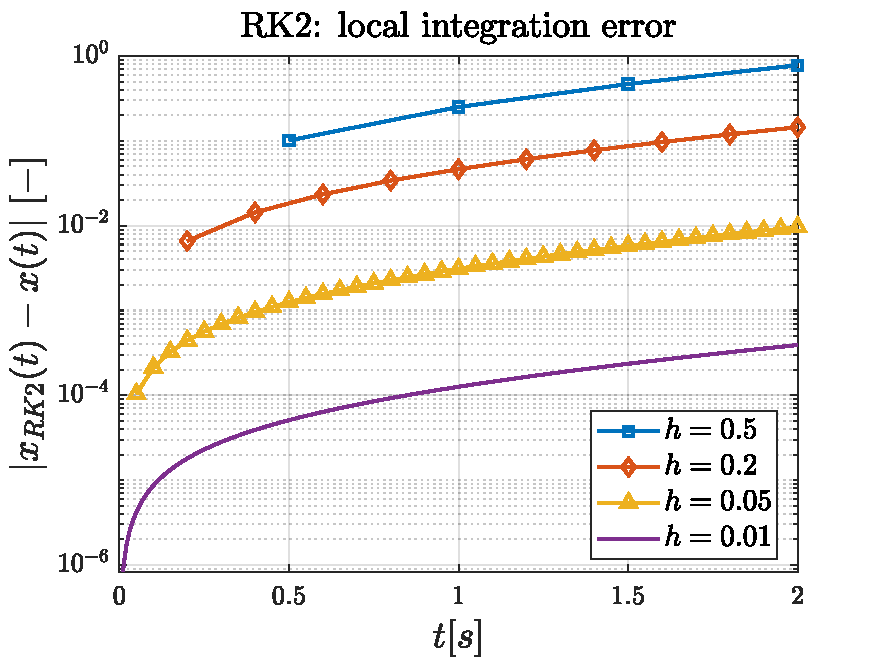
\includegraphics[width = 0.48\textwidth]{gfx/ex2_3.pdf}
    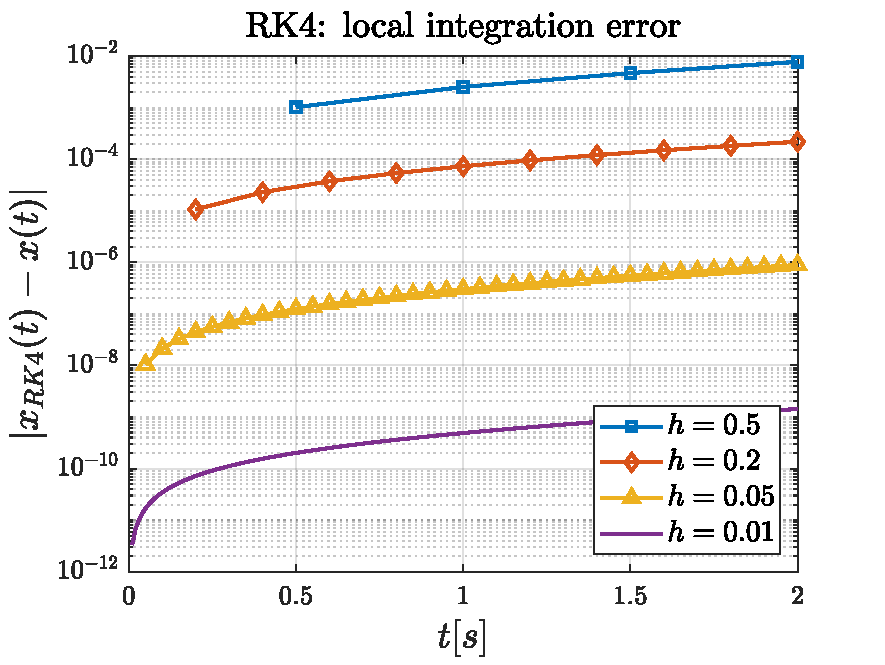
\includegraphics[width = 0.48\textwidth]{gfx/ex2_4.pdf}
    \caption{Local integration errors provided by with $RK2$ (left) and $RK4$ (right) methods by varying $h$ value.}
    \label{fig:ex2_locErr}
\end{figure}

\begin{figure}[h]
    \centering
    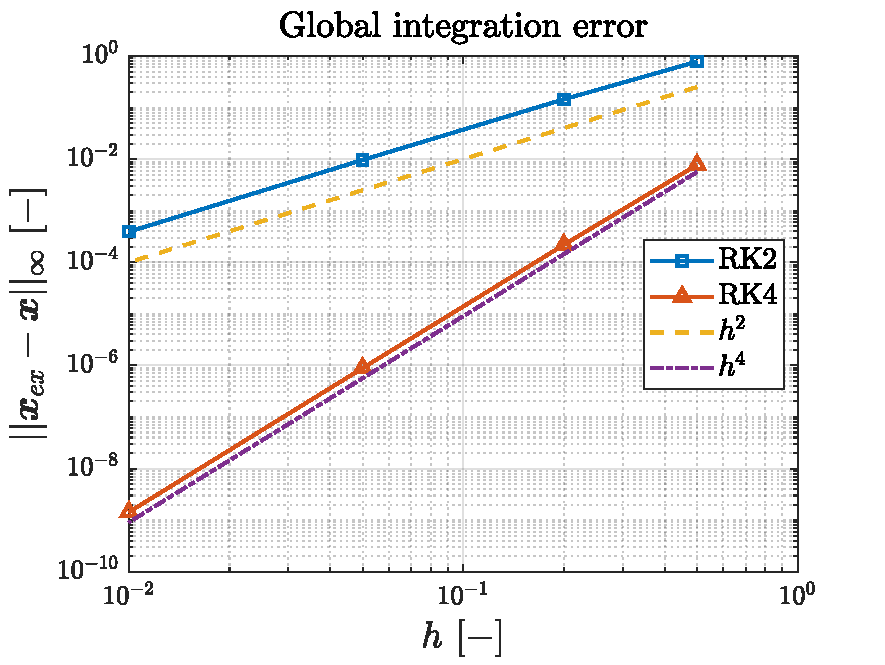
\includegraphics[width = 0.48\textwidth]{gfx/ex2_5.pdf}
    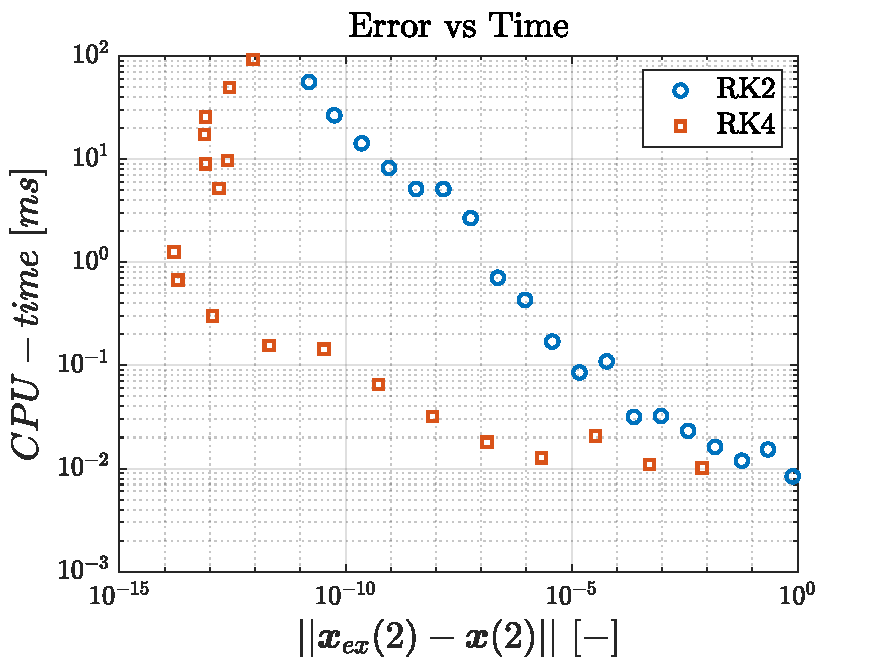
\includegraphics[width = 0.48\textwidth]{gfx/ex2_6.pdf}
    \caption{Global integration errors (left) and comparison between error and computational time of RK2 and RK4 methods (right).}
    \label{fig:ex2_globErr}
\end{figure}



\subsection*{Exercise 3}

Let $\dot{\vec x} = A(\alpha) \vec x$ be a two-dimensional system with $A(\alpha) = [0, 1; -1, 2\cos\alpha]$. Notice that $A(\alpha)$ has a pair of complex conjugate eigenvalues on the unit circle; $\alpha$ denotes the angle from the $\operatorname{Re}\{\lambda\}$-axis. 
\begin{enumerate*}[label=\arabic*)]
    \item Write the operator $F_{\rm RK2}(h,\alpha)$ that maps $\vec x_k$ into $\vec x_{k+1}$, namely $\vec x_{k+1} = F_{\rm RK2}(h,\alpha) \, \vec x_k$.
    \item\!With $\alpha = \pi$, solve the problem ``Find $h\ge 0$ s.t.$\max\left(|{\rm eig}(F(h,\alpha))|\right) = 1$''.
    \item Repeat point 2) for $\alpha\in[0, \pi]$ and draw the solutions in the $(h\lambda)$-plane.
    \item Repeat points 1)--3) with RK4.
\end{enumerate*}

\rightline{\small(5 points)}
\medskip \hrule \medskip

In order to retrieve the expression of the linear operator $F_{RK2}(h,\alpha)$ a generic RK2 iteration with step h is derived:
\begin{equation}
    \begin{cases}
        \vec{x}_{k+1}^P = \vec{x}_k + h\vec{f}(\vec{x}_k, t_k)\\
        \vec{x}_{k+1} = \vec{x}_k + \frac{h}{2}[\vec{f}(\vec{x}_k,t_k)+\vec{f}(\vec{x}_{k+1}^P, t_{k+1})]
    \end{cases}
    \label{eq:wow}
\end{equation}
where, in our case, $\vec{f}(\vec{x}_k, t_k) = \vec{A}(\alpha)\vec{x}_k$. By substituting the 
first equation of \autoref{eq:wow} in the second one it is obtained:
\begin{equation}
    \vec{x}_{k+1} = \vec{x}_k + \frac{h}{2}\vec{A}(\alpha)\vec{x}_k + \frac{h}{2}\vec{A}(\alpha)\vec{x}_k + \frac{h}{2}h\vec{A}(\alpha)^2\vec{x}_k
\end{equation}
By rearranging:
\begin{equation}
    \vec{x}_{k+1} = (\vec{I} + h\vec{A}(\alpha) + \frac{h^2}{2}\vec{A}^2(\alpha))\vec{x}_k = \vec{F}_{RK2}(h,\alpha)\vec{x}_k
\end{equation}
The same procedure can be performed to find $F_{RK4}$:
\begin{equation}
    \vec{F}_{RK4}(h,\alpha) = \vec{I} + h\vec{A}(\alpha) + \frac{h^2}{2}\vec{A}^2(\alpha) +  \frac{h^3}{6}\vec{A}^3(\alpha) + \frac{h^4}{24}\vec{A}^4(\alpha)
\end{equation}
\autoref{tab:ex3_ris} shows the solutions of the statement ``
Find $h\ge 0$ s.t.$\max\left(|{\rm eig}(F(h,\alpha))|\right) = 1$'' 
imposing $\alpha=\pi$ with both $F_{RK2}$ and $F_{RK4}$.
\begin{table}[h]
    \centering
    \begin{tabular}{l | c c}
         & $\vec{RK2}$ &  $\vec{RK4}$\\
        \midrule \midrule
        h & 2.0000000 & 2.7852935
    \end{tabular}
    \caption{Results of statement ``Find $h\ge 0$ s.t.$\max\left(|{\rm eig}(F(h,\alpha))|\right) = 1$'' where  $\alpha=\pi$ with $F_{RK2}$ and $F_{RK4}$ functions.}
    \label{tab:ex3_ris}
\end{table}

By solving the problem for $\alpha\in[0, \pi]$ the domain of numerical stability of bot RK2 
and RK4 methods is retrieved and plotted in \autoref{fig:ex3_stab}. A shown in the figure, 
the stability domains grow with increasing approximation order and higher-order algorithms 
call for larger step sizes.

\begin{figure}[h]
    \centering
    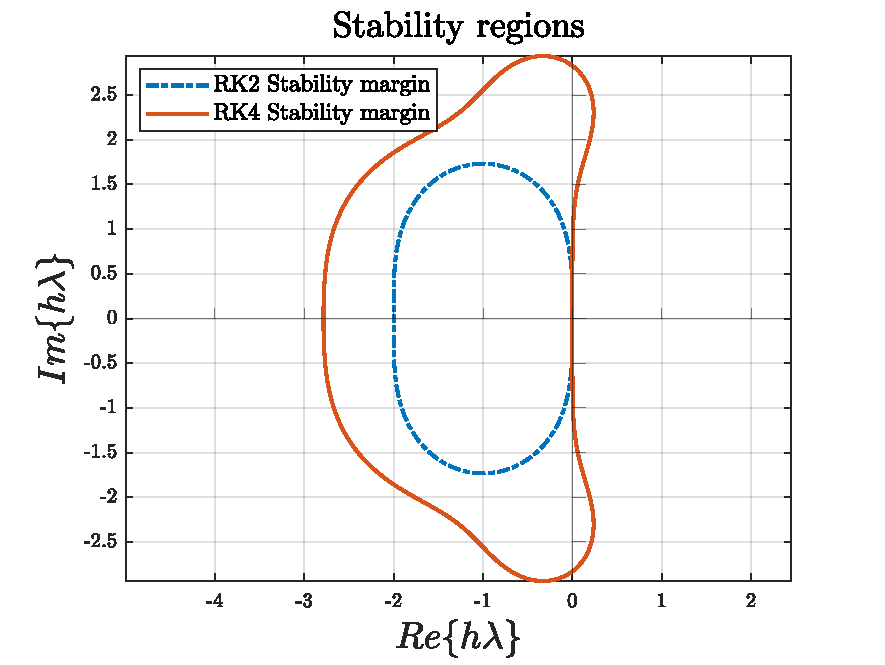
\includegraphics[width=0.49\textwidth]{gfx/ex3_2.pdf}
    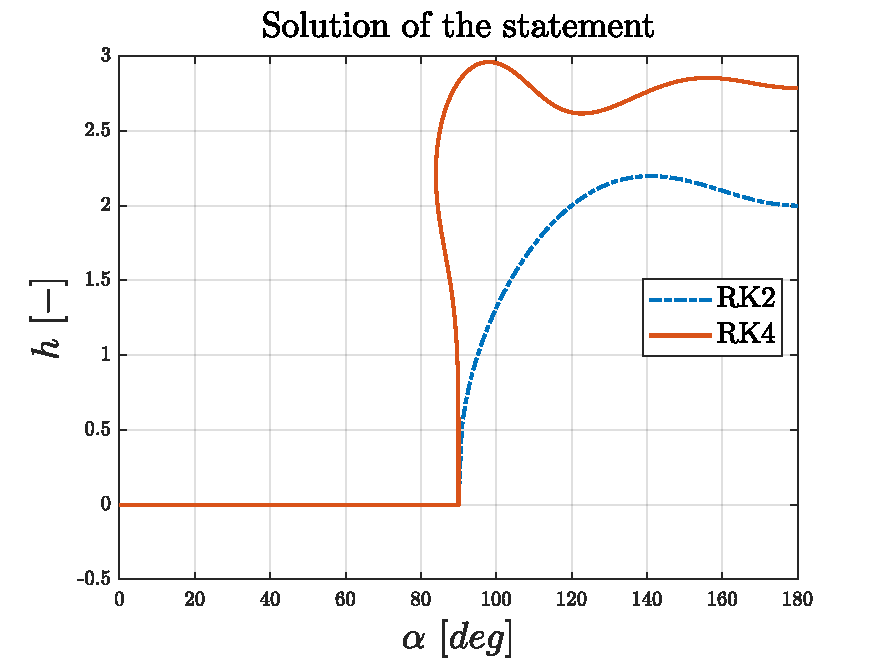
\includegraphics[width=0.49\textwidth]{gfx/ex3_1.pdf}
    \caption{RK2 and RK4 method stability domain (left) and solution of the statement ``Find $h\ge 0$ s.t.$\max\left(|{\rm eig}(F(h,\alpha))|\right) = 1$'' with RK2 and RK4 (right).}
    \label{fig:ex3_stab}
\end{figure}

\subsection*{Exercise 4}

Consider the IVP $\dot{\vec x}=A(\alpha)\vec x$, $\vec x(0) = [1, 1]^T$, to be integrated in $t\in[0, 1]$.
\begin{enumerate*}[label=\arabic*)]
    \item Take $\alpha\in[0, \pi]$ and solve the problem ``Find $h\ge 0$ s.t. $\left\|\vec x_{\rm an}(1)-\vec x_{\rm RK1}(1)\right\|_\infty = \mathrm{tol}$'', where $\vec x_{\rm an}(1)$ and $\vec x_{\rm RK1}(1)$ are the analytical and the numerical solution (with RK1) at the final time, respectively, and $\rm tol = \{10^{-3}, 10^{-4}, 10^{-5}, 10^{-6}\}$.
    \item Plot the four locus of solutions in the $(h\lambda)$-plane; plot also the function evaluations vs tol for $\alpha= \pi$.
    \item Repeat points 1)--2) for RK2 and RK4.
\end{enumerate*}

\rightline{\small(4 points)}
\medskip \hrule \medskip

Results are shown in \autoref{fig:ex4_1} and in \autoref{fig:ex4_2}. As the figure depicts, higher order approximation 
methods implies larger admissible values of step $h$. As a result, to grant the same tolerance 
of the error $\left\|\vec x_{\rm an}(1)-\vec x_{\rm RK1}(1)\right\|_\infty$, higher order 
methods can afford larger $h$ which results in less step in which the function must be 
evaluated. Last figure of \autoref{fig:ex4_2} demonstrates this fact.
\begin{figure}[h]
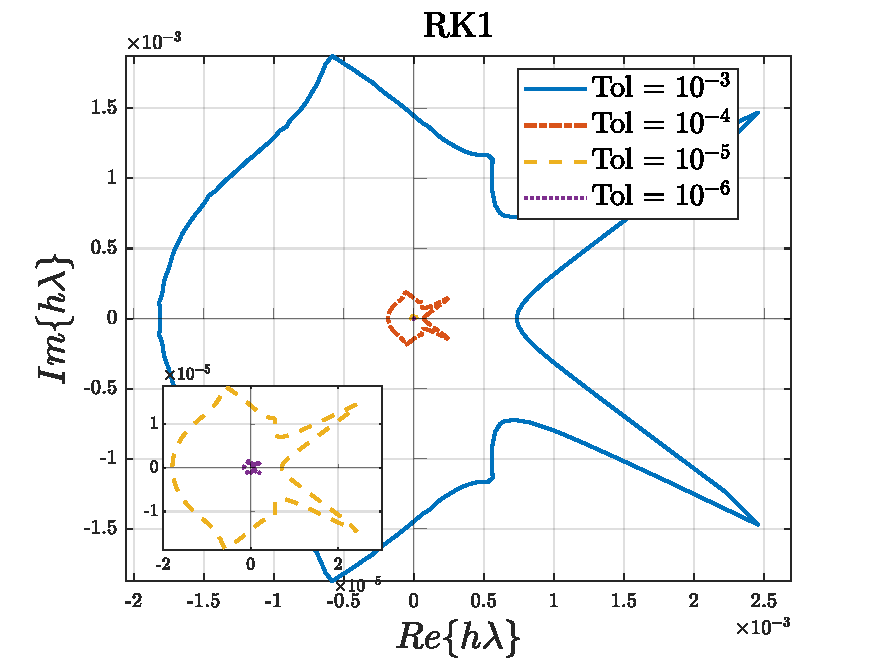
\includegraphics[width=0.48\textwidth]{gfx/ex4_1.pdf}
    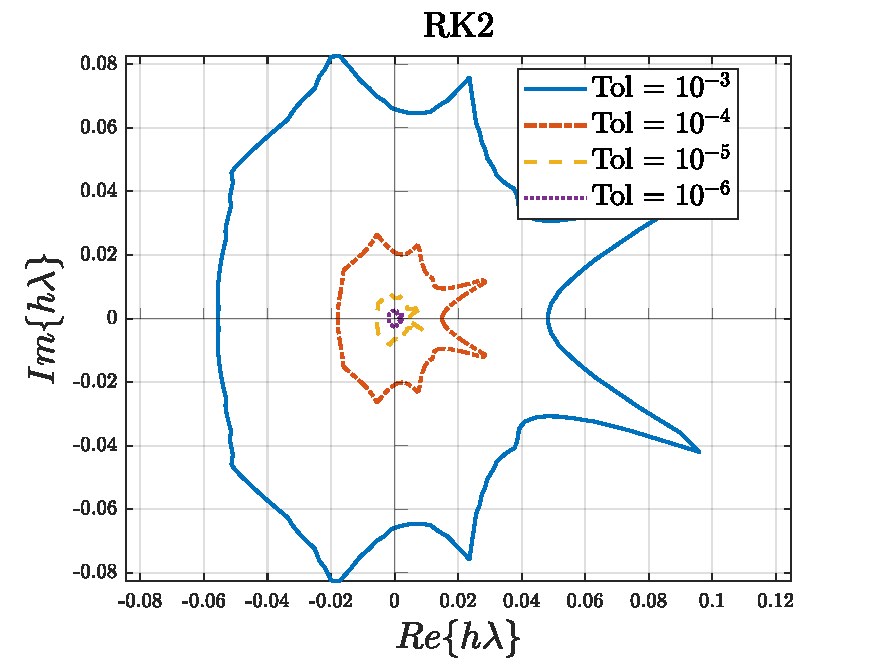
\includegraphics[width=0.48\textwidth]{gfx/ex4_2.pdf}
    \caption{Five locus of solutions for RK1 (left) and RK2 (right) methods.}
    \label{fig:ex4_1}
\end{figure}
\begin{figure}[h]
    \centering
    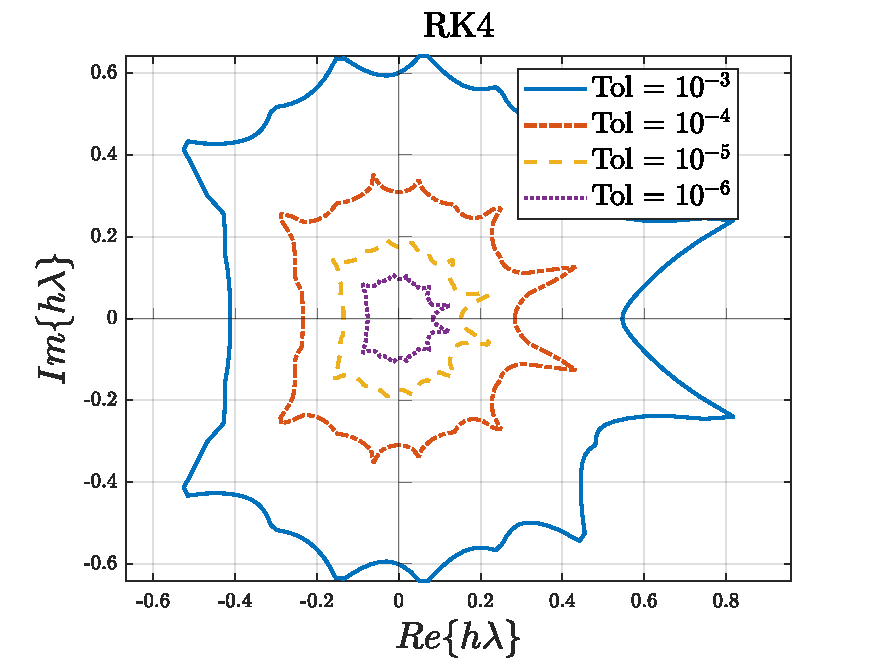
\includegraphics[width=0.48\textwidth]{gfx/ex4_3.pdf}
    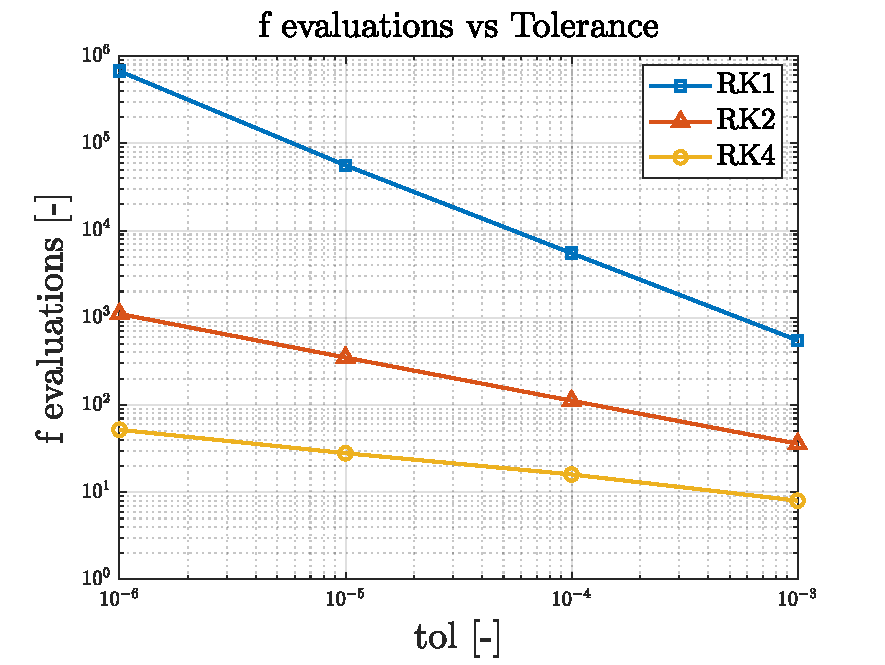
\includegraphics[width=0.48\textwidth]{gfx/ex4_4.pdf}
    \caption{RK4 locus of solutions (left) and function evaluations vs. tolerance (right).}
    \label{fig:ex4_2}
\end{figure}


\subsection*{Exercise 5}
Consider the backinterpolation method $\textrm{BI2}_{0.4}$. 1) Derive the expression of the 
linear operator $B_{\rm BI2_{0.4}}(h,\alpha)$ such that $\vec x_{k+1} = B_{\rm BI2_{0.4}}(h,\alpha) \vec x_k$. 2) 
Following the approach of point 3) in Exercise 3, draw the stability domain of 
$\textrm{BI2}_{0.4}$ in the $(h\lambda)$-plane. 3) Derive the domain of numerical stability 
of $\textrm{BI2}_{\theta}$ for the values of $\theta = [0.1,\, 0.3,\, 0.7,\, 0.9]$.

\rightline{\small(5 points)}
\medskip \hrule \medskip

\tr{\textit{Write your answer here}}

\subsection*{Exercise 6}

Consider the IVP $\dot{\vec x} = B \vec x$ with $B =[-180.5, 219.5; 179.5, -220.5]$ and $\vec{x}(0)=[1, 1]^T$ to be integrated in $t\in[0, 5]$. Notice that $\vec{x}(t)=e^{Bt}\vec{x}(0)$.
\begin{enumerate*}[label=\arabic*)]
    \item Solve the IVP using RK4 with $h=0.1$;
    \item Repeat point 1) using implicit extrapolation technique IEX4;
    \item Compare the numerical results in points 1) and 2) against the analytic solution;
    \item Compute the eigenvalues associated to the IVP and represent them on the $(h\lambda)$-plane both for RK4 and IEX4;
    \item Discuss the results.
\end{enumerate*}

\rightline{\small(4 points)}
\medskip \hrule \medskip

\tr{\textit{Write your answer here}}


\subsection*{Exercise 7}

Consider the two-dimensional IVP 
$$\begin{bmatrix}\dot{x}_1 \\ \dot{x}_2\end{bmatrix}=\begin{bmatrix}-\frac{5}{2}\left[1+8\sin(t)\right]x_1 \\ (1-x_1)x_2+x_1\end{bmatrix}, \qquad \begin{bmatrix} x_1(t_0)\\ x_2(t_0)\end{bmatrix}=\begin{bmatrix} 1\\ 1\end{bmatrix}$$
\begin{enumerate*}[label=\arabic*)]
    \item Solve the IVP using AB3 in $t\in[0,3]$ for $h=0.1$;
    \item Repeat point 1) using AM3, ABM3, and BDF3;
    \item Discuss the results.
\end{enumerate*}

\rightline{\small(5 points)}
\medskip \hrule \medskip



\tr{\textit{Write your answer here}}



\end{document}

%--------------------------------------------------------------------------------
%       END DOCUMENT
%--------------------------------------------------------------------------------